\documentclass[Space3_Assign1.tex]{subfiles}

\begin{document}

\section{Simulation of Orbits with Classical Elements}
\subsection{Introduction}
- keplers three laws\\
- perifocal frame\\
- The true anomaly $\theta$ is the angle taken at the focus of the perifocal frame to the satellite from the perigee. The eccentric anomaly $\textit{E}$ is the angle taken at the centre of perifocal frame to the satellite from the perigee.\\
-The mean anomaly \textit{$M_t$} is the mean number of orbits per day.\\
- LEO,MEO\\
-TLE's \\



\subsection{Methodology}
From Kepler's second law, the mean anomaly at time $\textit{t}$ is calculated using the mean motion $\textit{n}$ from an epoch time described by $M_0(t_0)$. 
\begin{eqnarray}
M_t = M_0 + n(t-t_0)
\end{eqnarray}
To solve for the eccentric anomaly, newtons method was used
\begin{eqnarray}
E_{i+1} &=& E_i - \frac{f(E_i)}{f'(E_i)}\\
E_{i+1} &=& E_i - \frac{E-e\sin(E_i)-M_t}{1-e\cos(E_i)}
\end{eqnarray}
The true anomaly was calculated using
\begin{equation}
\theta = 2\tan^{-1}\left(\sqrt{\frac{1+e}{1-e}}\tan\left(\frac{E}{2}\right)\right)
\end{equation} 
The general equation for the radius of an ellipse
\begin{eqnarray}
r = \frac{p}{1+e\cos\theta}
\end{eqnarray}
The two parameters, $\theta$ and r can completely define the orbit in the perifocal frame as polar coordinates. The conversion to cartesian coordinates in the perifocal frame are as follows:
\begin{eqnarray}
\left[ \begin{array}{c}
x\\y\\z
\end{array} \right]_{perifocal} &=& \left[ \begin{array}{c}
r\cos\theta \\ r\sin \theta \\ 0
\end{array} \right] \\
\left[ \begin{array}{c}
v_x\\v_y\\v_z
\end{array} \right]_{perifocal} &=& \left[ \begin{array}{c}
-\sqrt{\frac{\mu}{p}}\sin\theta \\\sqrt{\frac{\mu}{p}}(e+\cos\theta) \\ 0
\end{array} \right] \\
\end{eqnarray}
The perifocal parameters were transformed to the ECI frame to animate the 3D model of the satellite orbit around the Earth using the function \textit{\textbf{orbit2ECI}}. From the ECI coordinates, the ECEF and LLHGD coordinates were calculated for the ground trace.



\subsubsection{Orbital Period}
The period was calculated analytically and computationally. The period is inversely proportional to the mean motion. From the simulation, the ECI coordinates of the satellite were analysed by auto correlation based on the Wiener-Khinchin Theorem. The data was fast fourier transformed using the built-in matlab function, multiplied with the resultant complex conjugate then transformed back to the time domain by inverse fourier transform. 
\lstinputlisting{../Assignment1/Subfns/Period_AC.m}

\subsection{Results/Discussion}
\subsubsection{Van Allen Probes}
The satellites Van Allen Probes, previously known as the Radiation Belt Storm Probes (RBSP A and B), are in a highly eccentric orbit. RBSP-A was modelled based on TLEs from spacetrack.com, see Table \ref{Q1.orbitprop}. It was launched on 30th August 2012 

The Van Allen Belts are regions of plasma that surround the Earth that are contained by the Earth's magnetic field. The highly energetic particles become trapped in the Earth's magnetic field by travelling along the field lines to a pole and being reflected back and travelling to the opposite pole. This phenomenon is called a magnetic mirror, and is the reason the Van Allen belts have a torus shape about the Earth's magnetic axis, see Figure \ref{fig:VanAllenNASA}. Therefore, the radiation is at the highest intensity about the magnetic equatorial plane, currently at 11.5$^{\circ}$ inclination. The satellite was put in an orbit close to this inclination at about 10$^{\circ}$, with the mission objective to be in an orbit of no greater than 18$^{\circ}$. The inclination has fluctuated between 9-11$^{\circ}$ over the course of it's mission.

The orbit was highly eccentric in order to cover the entire radiation belt region. The perigee altitude is 500 km, which is below the inner radiation belt and the apogee altitude is 30600 km, which is above the outer edge of the outer radiation belt.
\begin{figure}
\centering
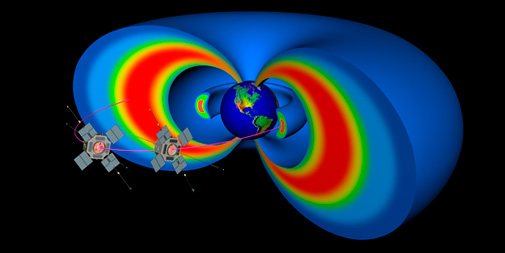
\includegraphics[width=0.7\linewidth]{VanAllenNASA}
\caption{}
\label{fig:VanAllenNASA}
\end{figure}

% http://www.scf.jhuapl.edu/
\subsubsection{Solar Radiation and Climate Experiment (SORCE)}
- long term measurements of total solar irradiance in UV and VNIR
- how and why variability occurs at the sun and how it affects our atmosphere and climate
- launched in 2003
\subsubsection{Orbital Properties}
\begin{table}[h]
\centering
\caption{Orbital properties of simulated satellites. (* indicates data taken directly from TLEs)}
\label{Q1.orbitprop}
\begin{tabular}{|l|c|c|c|c|}
	\hline
	Orbital Properties              & Variable Name &     Units      & Van Allen Probe A &     SORCE      \\ \hline
	NORAD ID                        &               &                &                   &      27651       \\ \hline
	*Julian year/day data was taken &      t0       &    year/day    & 2016 68.37507029  & 2016 82.69823837 \\ \hline
	Semimajor axis                  &       a       &       m        &                   &  \\ \hline
	*Eccentricity                   &       e       &       -        &     0.6813430     &    0.0024311     \\ \hline
	*Inclination angle              &      inc      &    degrees     &      10.1687      &      39.9961      \\ \hline
	*Right ascension of the node    &     Rasc      &    degrees     &      46.5607      &     317.0592     \\ \hline
	*Argument of Perigee            &     omega     &    degrees     &      77.2770      &     301.6655     \\ \hline
	*Mean Anomaly                   &      Mt       &    degrees     &     346.0491      &     58.1763      \\\hline
	*Mean Motion             &      MM       & orbits per day &    2.681033090    &     14.88275952      \\ \hline
	Analytical Period               &               &                &                   &  \\ \hline
	Computational Period            &               &                &                   &  \\ \hline
	Altitude at Perigee             &               &                &                   &  \\ \hline
	Altitude at Apogee              &               &                &                   &  \\ \hline
\end{tabular}
\end{table}

% The Van Allen Probes Mission
%Nicola Fox, James L. Burch
%Springer Science & Business Media, 10Jan.,2014 - Science - 647 pages
\end{document}